%\chapter{Concept}
\chapter{Catching Attackers in a Restricted Network Area}
\label{chap:concept}

\section{Introduction}

\section{Heidelberg Connection Acceptance Tool}

MADCAT stand for Mass Attack Detection Connection Acceptance Tools and works as a honeypot-like detection application with low interaction-level. 

\begin{figure}[ht]
    \centering
    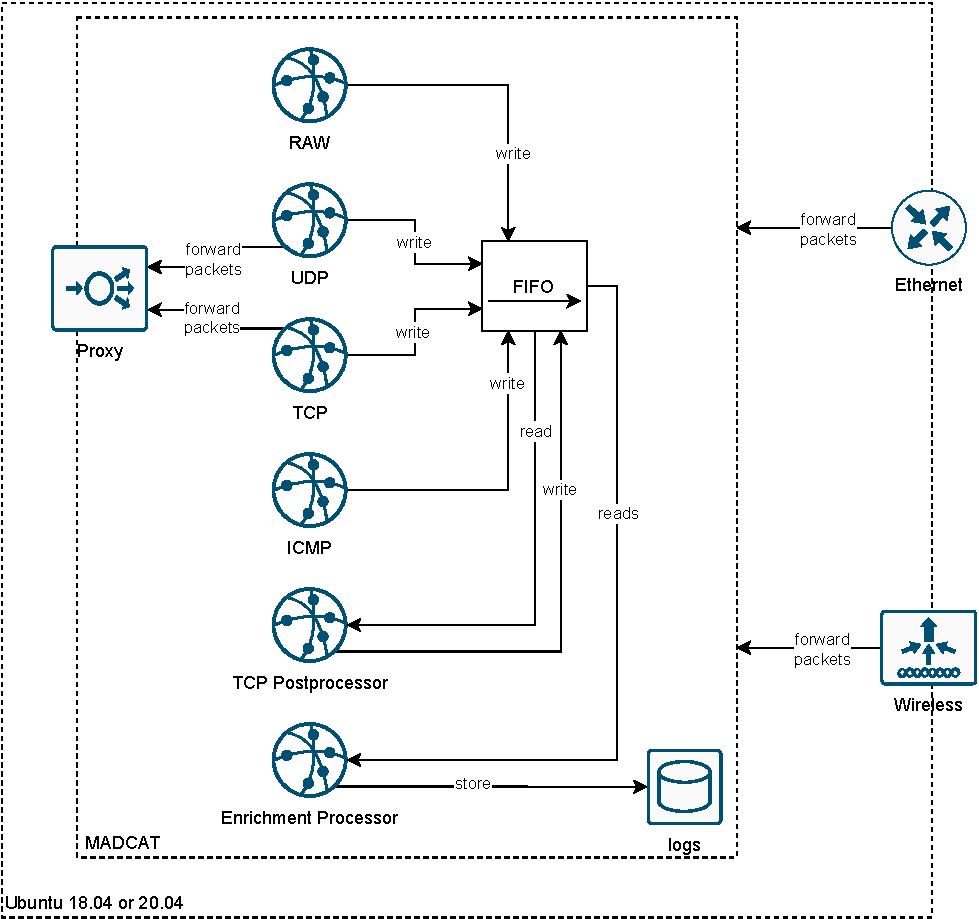
\includegraphics[width=\textwidth]{figures/heicat-architecture.pdf}
    \caption[MADCAT architecture.]{MADCAT architecture. The Ethernet and wireless interface forwards the respective packets to the desired module.}
    \label{fig:heicat-architecture}
\end{figure}

Our idea to catch any connection acquired to our honeypot is carried out in \autoref{fig:heicat-concept}.

\begin{figure}[ht]
    \centering
    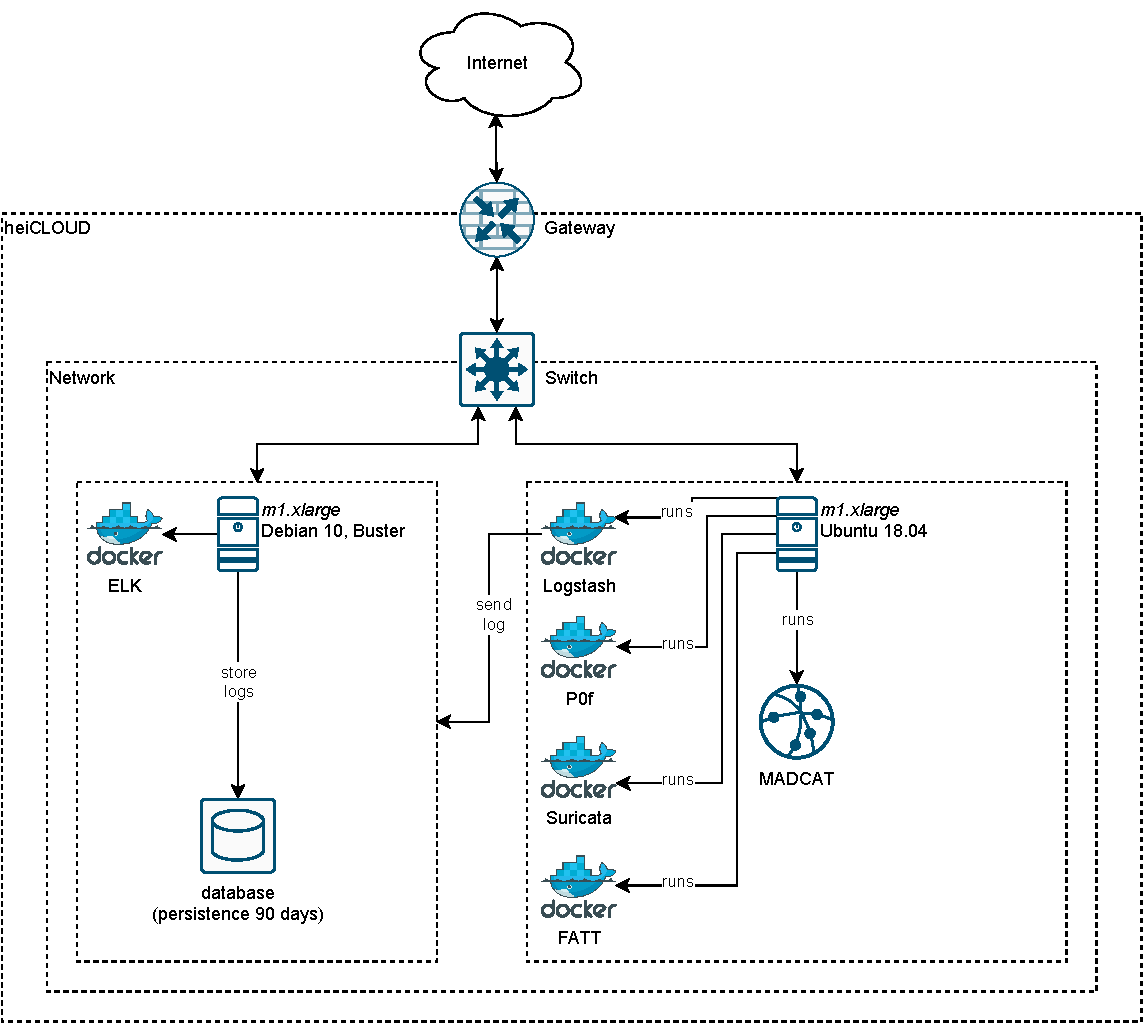
\includegraphics[width=\textwidth]{figures/heicat-conecpt.pdf}
    \caption[HeiCAT concept]{HeiCAT concept.}
    \label{fig:heicat-concept}
\end{figure}

\section{Results}
